%!TEX root = ../../../thesis.tex

\section{Phosphate Buffered Saline}
    \subsection{Resistor Mesh}
        The two stimulus electrodes were driven at \SI{500}{\micro\ampere} at a frequency of \SI{10}{\kilo\hertz}.

    \subsection{Series Resistance And Constant Phase Element}
        Discuss equipment and settings used to make the measurements.

        \begin{figure}
          \centering
          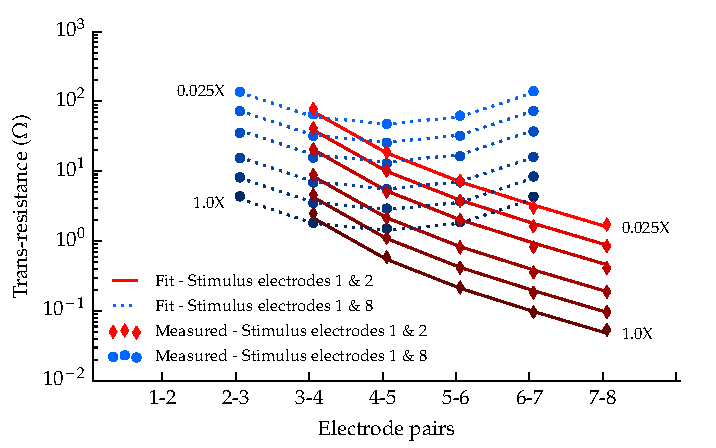
\includegraphics{content/pt2/07-InterfaceModel/graphics/graph_transimpedance_pbs}
          \caption{\label{fig:pt2-graph_transimpedance_pbs}Measured and fitted values of trans-impedance for both measurement configurations. Voltage measurements are made between adjacent pairs of electrodes as current is pushed through the stimulus electrodes.}
        \end{figure}

        \Cref{fig:pt2-graph_transimpedance_pbs} shows measurement results for each pair of non-stimulated pair of electrodes along with simulated results using the fitted parameters.


        \begin{table}
          \centering
          \begin{tabular}{r | l}
            Parameter & Value \\
            \hline
            $R_{eri}$ ($\Omega$)& 0.407 / $\sigma$\\
            $R_{sri}$ ($\Omega$)& $R_{eri}\cdot 3/4$\\
            $R_{li}$ ($\Omega$)& 3.71 / $\sigma$ \\
            Depth (layers) & 5 \\
            Padding (layers) & 3 \\
          \end{tabular}
          \caption{\label{tab:RESparams}Resistor mesh parameters. Electrolyte conductivity ($\sigma$) is expressed in units of $S / cm$}
        \end{table}

    \subsection{Faradaic Current}

        Faradaic processes at an electrode/electrolyte interface are modeled
        by the Butler-Volmer equation:

        \begin{equation}
        i_{net}=i_{o}\left\{ \frac{[O]_{(0,t)}}{[O]_{\infty}}e^{\frac{-\alpha_{c}nF\eta}{RT}}-\frac{[R]_{(0,t)}}{[R]_{\infty}}e^{\frac{(1-\alpha_{c})nF\eta}{RT}}\right\}
        \end{equation}


        where:

        \begin{tabular}{rl}
        $i_{net}$ & = net Faradaic current\tabularnewline
        $i_{o}$ & = current exchange density\tabularnewline
        $[O]_{(0,t)}$ & = concentration of oxidising species at electrode surface $(x=0)$\tabularnewline
        $[R]_{(0,t)}$ & = concentration of reducing species at the electrode surface\tabularnewline
        $[O]_{\infty}$ & = bulk concentration of oxidising species in electrolyte\tabularnewline
        $[R]_{\infty}$ & = bulk concentration of oxidising species in electrolyte\tabularnewline
        $\alpha_{c}$ & = cathodic transfer coefficient\tabularnewline
        $n$ & = number of moles of electrons per mole of reactant oxidised\tabularnewline
        F & = Faraday's constant $\approx96,485$\tabularnewline
        R & = the gas constant $\approx8.314$\tabularnewline
        T & = absolute temperature in Kelvin\tabularnewline
        $\eta$ & = electrode overpontential\tabularnewline
        \end{tabular}


    \subsection{Final Model}

\section{Biological parameter measurements}
    \label{sect:sheep_measurements}
    \subsection{Resistor Mesh}
    \subsection{Series Resistance And Constant Phase Element}
    \subsection{Faradaic Current}
    \subsection{Final Model}

